%% This is file `elsarticle-template-1-num.tex',
%%
%% Copyright 2009 Elsevier Ltd
%%
%% This file is part of the 'Elsarticle Bundle'.
%% ---------------------------------------------
%%
%% It may be distributed under the conditions of the LaTeX Project Public
%% License, either version 1.2 of this license or (at your option) any
%% later version.  The latest version of this license is in
%%    http://www.latex-project.org/lppl.txt
%% and version 1.2 or later is part of all distributions of LaTeX
%% version 1999/12/01 or later.
%%
%% The list of all files belonging to the 'Elsarticle Bundle' is
%% given in the file `manifest.txt'.
%%
%% Template article for Elsevier's document class `elsarticle'
%% with numbered style bibliographic references
%%
%% $Id: elsarticle-template-1-num.tex 149 2009-10-08 05:01:15Z rishi $
%% $URL: http://lenova.river-valley.com/svn/elsbst/trunk/elsarticle-template-1-num.tex $
%%
\documentclass[preprint,12pt]{elsarticle}

%% Use the option review to obtain double line spacing
%% \documentclass[preprint,review,12pt]{elsarticle}

%% Use the options 1p,twocolumn; 3p; 3p,twocolumn; 5p; or 5p,twocolumn
%% for a journal layout:
%% \documentclass[final,1p,times]{elsarticle}
%% \documentclass[final,1p,times,twocolumn]{elsarticle}
%% \documentclass[final,3p,times]{elsarticle}
%% \documentclass[final,3p,times,twocolumn]{elsarticle}
%% \documentclass[final,5p,times]{elsarticle}
%% \documentclass[final,5p,times,twocolumn]{elsarticle}

%% if you use PostScript figures in your article
%% use the graphics package for simple commands
%% \usepackage{graphics}
%% or use the graphicx package for more complicated commands
%% \usepackage{graphicx}
%% or use the epsfig package if you prefer to use the old commands
%% \usepackage{epsfig}
\usepackage[utf8]{vietnam}
\usepackage[vietnam]{babel}

%% The amssymb package provides various useful mathematical symbols
\usepackage{amssymb}
%% The amsthm package provides extended theorem environments
%% \usepackage{amsthm}

%% The lineno packages adds line numbers. Start line numbering with
%% \begin{linenumbers}, end it with \end{linenumbers}. Or switch it on
%% for the whole article with \linenumbers after \end{frontmatter}.
\usepackage{lineno}

%% natbib.sty is loaded by default. However, natbib options can be
%% provided with \biboptions{...} command. Following options are
%% valid:

%%   round  -  round parentheses are used (default)
%%   square -  square brackets are used   [option]
%%   curly  -  curly braces are used      {option}
%%   angle  -  angle brackets are used    <option>
%%   semicolon  -  multiple citations separated by semi-colon
%%   colon  - same as semicolon, an earlier confusion
%%   comma  -  separated by comma
%%   numbers-  selects numerical citations
%%   super  -  numerical citations as superscripts
%%   sort   -  sorts multiple citations according to order in ref. list
%%   sort&compress   -  like sort, but also compresses numerical citations
%%   compress - compresses without sorting
%%
%% \biboptions{comma,round}

% \biboptions{}


\journal{Journal Name}

\begin{document}

\begin{frontmatter}

%% Title, authors and addresses

%% use the tnoteref command within \title for footnotes;
%% use the tnotetext command for the associated footnote;
%% use the fnref command within \author or \address for footnotes;
%% use the fntext command for the associated footnote;
%% use the corref command within \author for corresponding author footnotes;
%% use the cortext command for the associated footnote;
%% use the ead command for the email address,
%% and the form \ead[url] for the home page:
%%
%% \title{Title\tnoteref{label1}}
%% \tnotetext[label1]{}
%% \author{Name\corref{cor1}\fnref{label2}}
%% \ead{email address}
%% \ead[url]{home page}
%% \fntext[label2]{}
%% \cortext[cor1]{}
%% \address{Address\fnref{label3}}
%% \fntext[label3]{}

\title{Report of Neural Machine Translation Model}

%% use optional labels to link authors explicitly to addresses:
%% \author[label1,label2]{<author name>}
%% \address[label1]{<address>}
%% \address[label2]{<address>}

\author{Huan Phan}

\address{VietAI Course 3's student, HCM, Vietnam}

\begin{abstract}
%% Text of abstract
XYZ
\end{abstract}

\begin{keyword}
Neural Machine Translation \sep Seq2Seq \sep Attention
%% keywords here, in the form: keyword \sep keyword

%% MSC codes here, in the form: \MSC code \sep code
%% or \MSC[2008] code \sep code (2000 is the default)

\end{keyword}

\end{frontmatter}

%%
%% Start line numbering here if you want
%%
\linenumbers

%% main text
\section{Overview of Neural Machine Translation}
\label{S:1}

\subsection{Encoder - Decoder Architect}

Trong mô hình seq2seq dùng cho bài toán NMT (Neural Machine Translation) bao gồm 2 mạng RNN chính: Encoder và Decoder. Encoder với đầu vào là câu ở ngôn ngữ gốc, đầu ra tại layer cuối cùng của Encoder gọi là 1 context vector. Với ý nghĩa lượng thông tin từ câu của Encoder sẽ được tóm gọn lại trong 1 vector đầu ra cuối cùng. Từ đó, Decoder dùng chính context vector đó, cùng với hidden state và từ trước đó để predict từ tiếp theo tại decoder qua từng timestep.

\begin{figure}[h]
\centering
\includegraphics[width=0.4\linewidth]{img/encdec.jpg}
\caption{Encoder-decoder architecture – example of a general approach for NMT. An encoder converts a source sentence into a "meaning" vector which is passed through a decoder to produce a translation.}
\end{figure}

\subsection{Neural Machine Translation Architect}

\begin{figure}[h]
\centering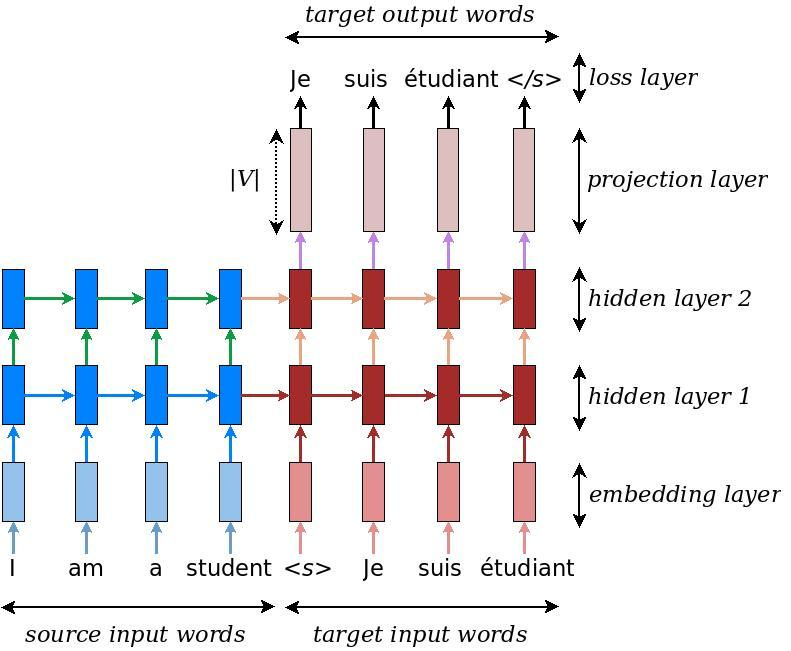
\includegraphics[width=0.4\linewidth]{img/seq2seq.jpg}
\caption{Neural machine translation – example of a deep recurrent architecture proposed by for translating a source sentence "I am a student" into a target sentence "Je suis étudiant". Here, "<s>" marks the start of the decoding process while "</s>" tells the decoder to stop.}
\end{figure}

\subsection{Attention Mechanise}

\textit{We conjecture that the use of a fixed-length vector is a
bottleneck in improving the performance of this basic encoder–decoder architecture, and propose to extend this by allowing a model to automatically (soft-)search for parts of a source sentence that are relevant to predicting a target word, without having to form these parts as a hard segment explicitly\cite{Bahdanau:2015}}

Việc encode toàn bộ thông tin từ source vào 1 vector cố định khiến việc mô hình khi thực hiện trên các câu dài (long sentence) không thực sự tốt, mặc dù sử dụng LSTM (BiLSTM, GRU) để khắc phục điểm yếu của mạng RNN truyền thống với hiện tượng Vanishing Gradient, nhưng như thế có vẻ vẫn chưa đủ, đặc biệt đối với những câu dài hơn những câu trong training data. Từ đó, trong paper, tác giả Bahdanau đề xuất 1 cơ chế cho phép mô hình có thể chú trọng vào những phần quan trọng (word liên kết với word từ source đến target), và thay vì chỉ sử dụng context layer được tạo ra từ layer cuối cùng của Encoder, tác giả sử dụng tất cả các output của từng cell qua từng timestep, kết hợp với hidden state của từng cell để "tổng hợp" ra 1 context vector (attention vector) và dùng nó làm đầu vào cho từng cell trong Decoder. 

\emph{Cơ chế "tổng hợp" Attention trong paper của tác giả Bahdanau: Align and Jointly model (Additive Attention).}

\begin{figure}[h]
\centering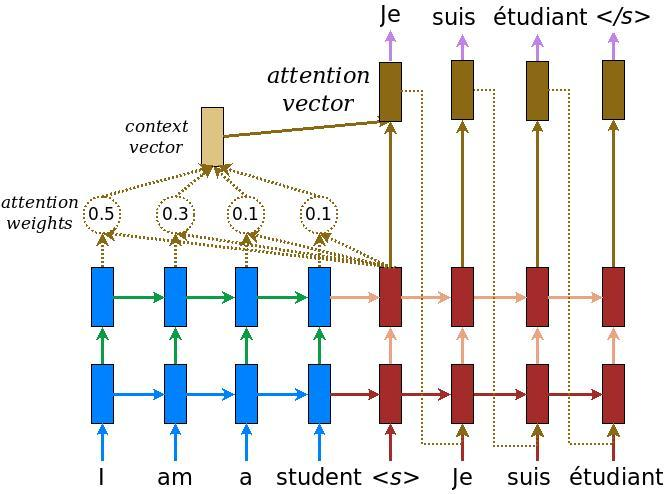
\includegraphics[width=0.4\linewidth]{img/attention_mechanism.jpg}
\caption{Attention mechanism – example of an attention-based NMT system as described in (Luong et al., 2015) . We highlight in detail the first step of the attention computation. For clarity, we don't show the embedding and projection layers in Figure (2).}
\end{figure}

Ma trận bất đối xứng (confusion matrix) được tạo ra bởi alignment score, thể hiện mức độ tương quan correlation giữa source và target.

\begin{figure}[h]
\centering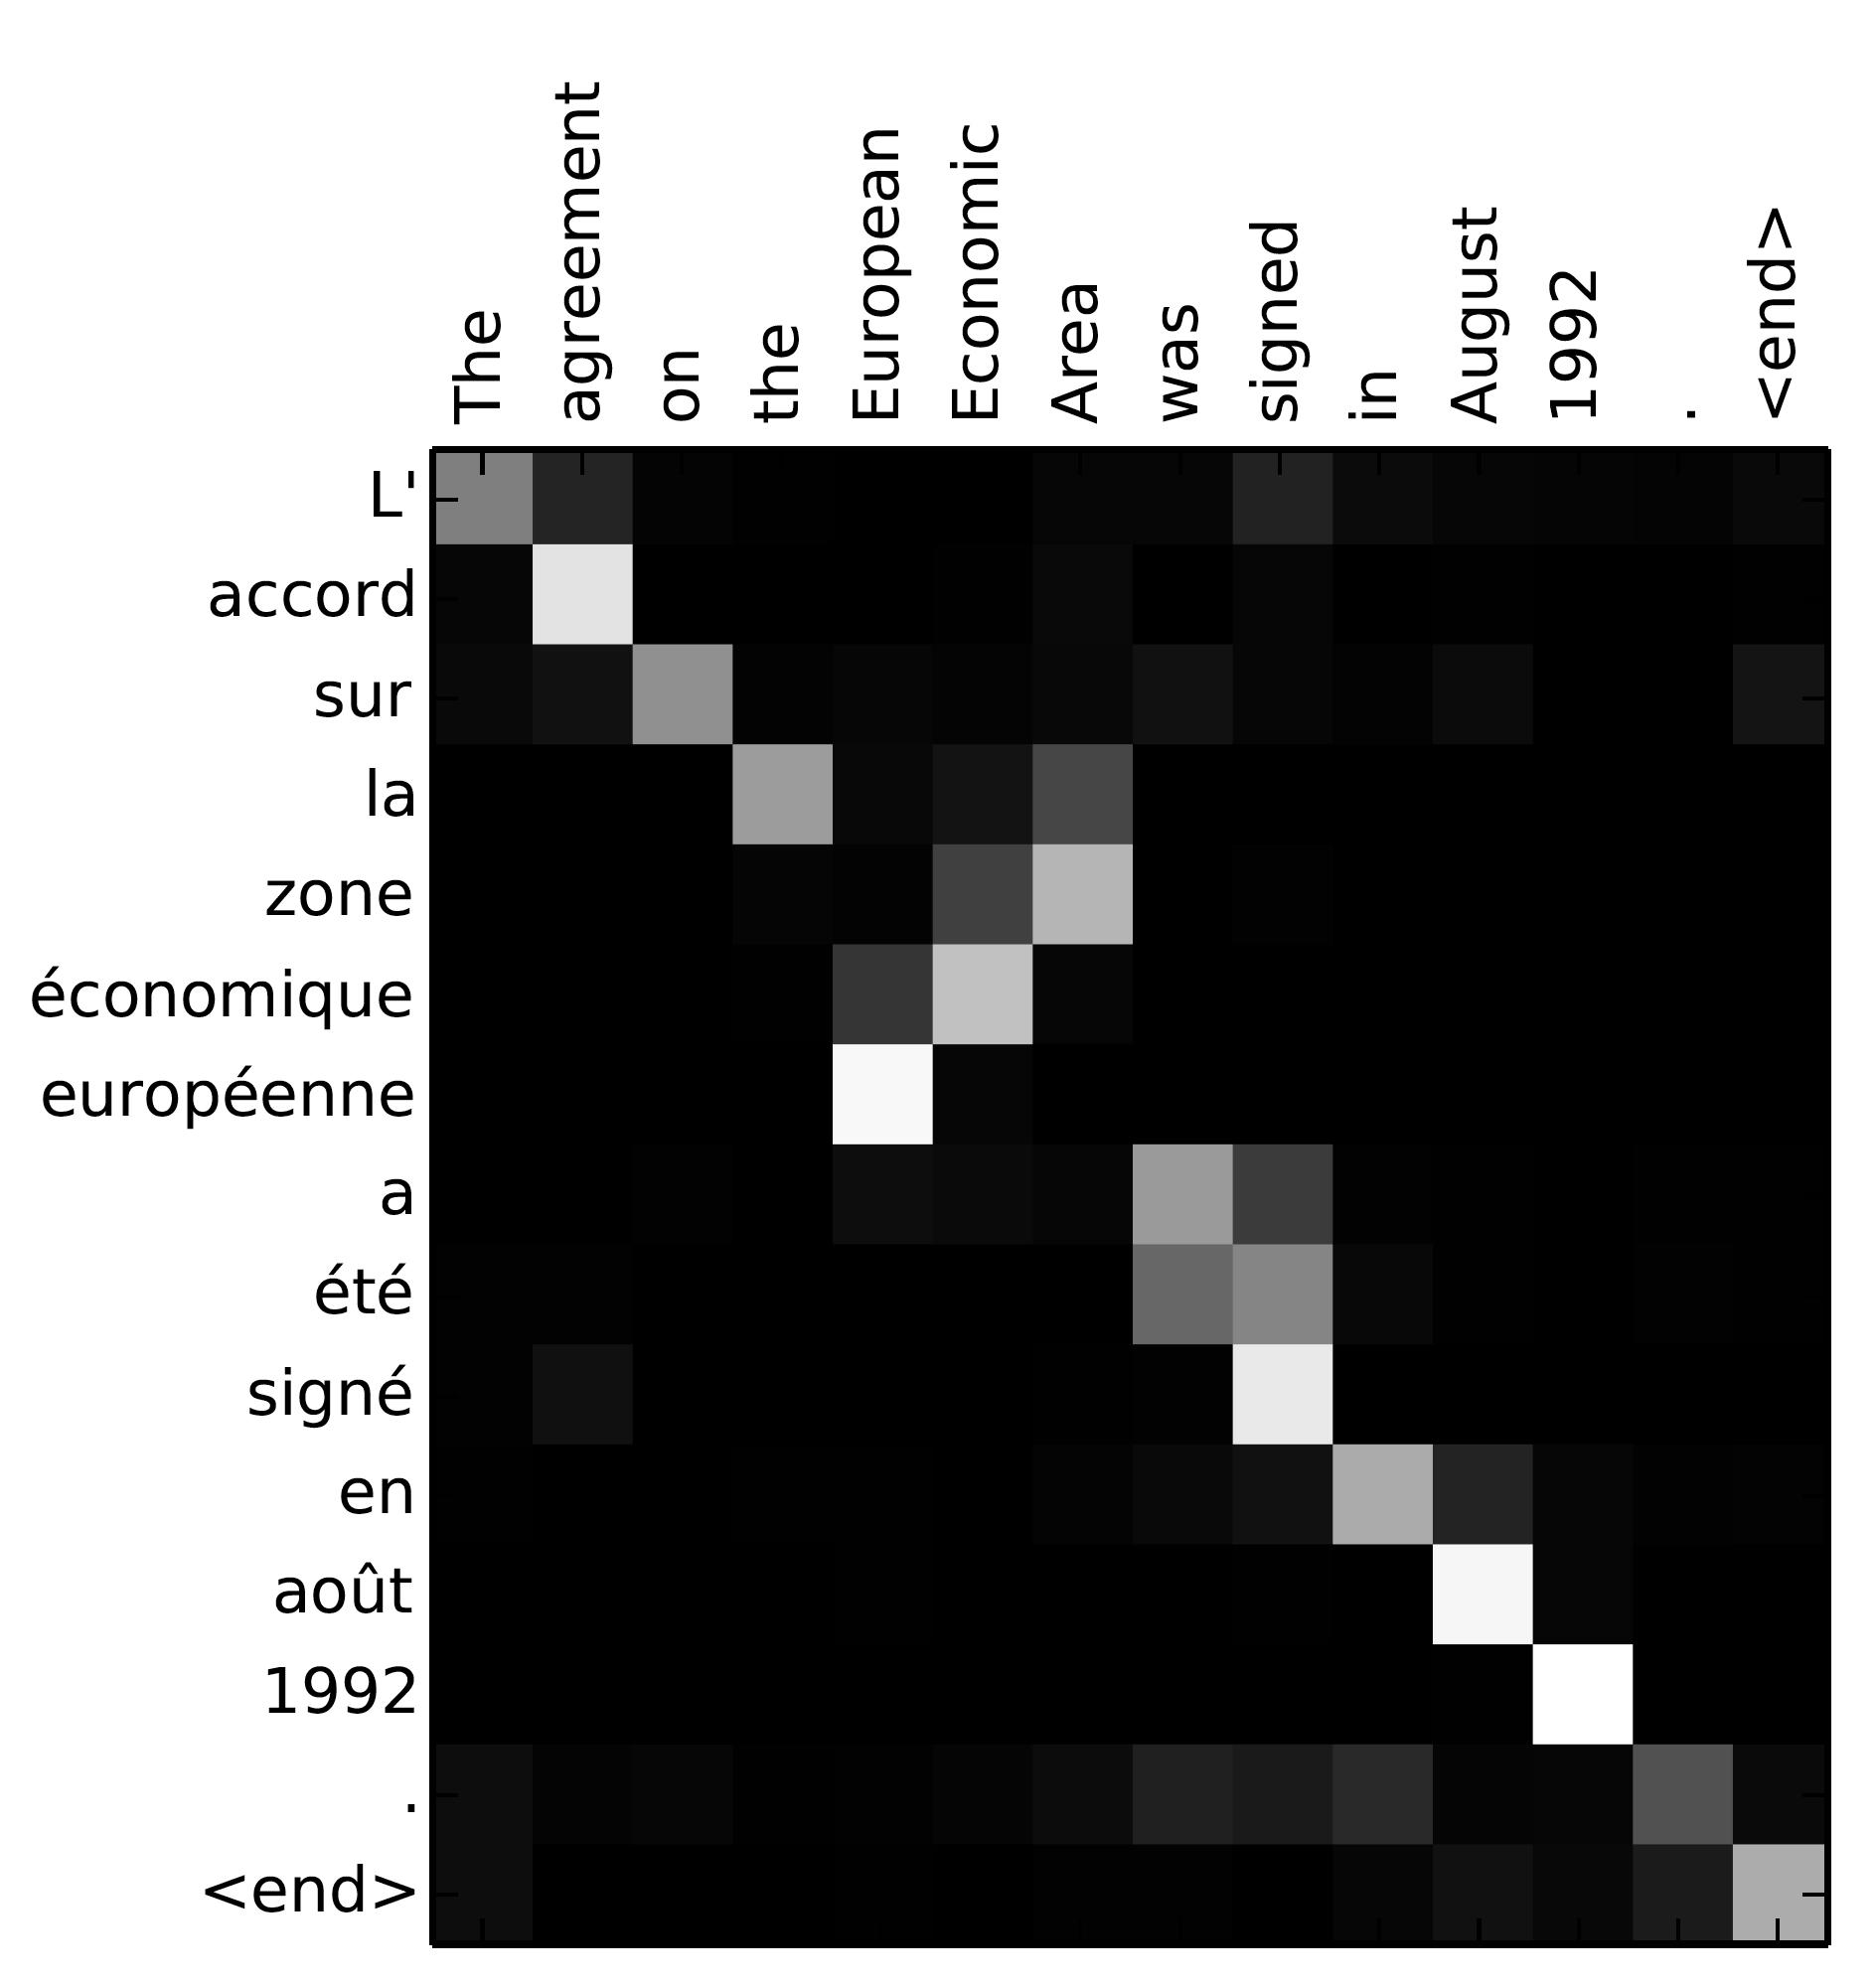
\includegraphics[width=0.4\linewidth]{img/attention_vis.jpg}
\caption{Attention visualization – example of the alignments between source and target sentences. Image is taken from (Bahdanau et al., 2015).}
\end{figure}

\subsection{(SGD, Adam)}

\subsection{Inference mode (Beam search, Greedy)}

\section{Measure performance with BLEU score}
\label{S:2}

\begin{equation}
\label{eq:emc}
e = mc^2
\end{equation}

\section{Training with different hyper-parameters}
\label{S:3}

\begin{table}[h]
\centering
\begin{tabular}{l l l}
\hline
\textbf{Treatments} & \textbf{Response 1} & \textbf{Response 2}\\
\hline
Treatment 1 & 0.0003262 & 0.562 \\
Treatment 2 & 0.0015681 & 0.910 \\
Treatment 3 & 0.0009271 & 0.296 \\
\hline
\end{tabular}
\caption{Table caption}
\end{table}


\section{Result with Attention Matrix}
\label{S:4}

%% The Appendices part is started with the command \appendix;
%% appendix sections are then done as normal sections
%% \appendix

%% \section{}
%% \label{}

%% References
%%
%% Following citation commands can be used in the body text:
%% Usage of \cite is as follows:
%%   \cite{key}          ==>>  [#]
%%   \cite[chap. 2]{key} ==>>  [#, chap. 2]
%%   \citet{key}         ==>>  Author [#]

%% References with bibTeX database:

\bibliographystyle{model1-num-names}
\bibliography{sample.bib}

%% Authors are advised to submit their bibtex database files. They are
%% requested to list a bibtex style file in the manuscript if they do
%% not want to use model1-num-names.bst.

%% References without bibTeX database:

% \begin{thebibliography}{00}

%% \bibitem must have the following form:
%%   \bibitem{key}...
%%

% \bibitem{}

% \end{thebibliography}


\end{document}

%%
%% End of file `elsarticle-template-1-num.tex'.
